\section{Grundlagen}
In diesem Kapitel werden die Grundlagen beleuchtet, auf denen diese Arbeit aufbaut. Zuerst wird auf die verwendeten Technologien eingegangen, die zum Einsatz kommen. Anschließend wird die Basisanwendung ViRGOS erklärt, die im Zuge dieser Arbeit erweitert wird. 

\subsection{Technologien}

In dieser Arbeit kommen hauptsächlich zwei Technologien zum Einsatz. Einerseits wird Unity als Entwicklungsumgebung benutzt, andererseits wird Photons PUN als Mehrspieler-Framework verwendet. 

\subsubsection*{Unity}
Unity ist eine Laufzeit- und Entwicklungsumgebung für die Entwicklung von 3D-Grafik-Anwendungen. Unity erlaubt das Entwerfen von 3D-Szenen. Es können Objekte in der Szene platziert, skaliert, verschoben, gedreht oder manipuliert werden. Eine Szene setzt sich aus GameObjects zusammen, die jeweils mit Komponenten versehen werden können. Somit kann beispielsweise dem GameObject eines Würfel eine Texturkomponente zugewiesen werden. Diese Komponente bestimmt dann das Aussehen der Oberfläche des Würfels. Um GameObjects zusätzliches Verhalten zu verleihen, das die eingebauten Mechanismen von Unity übersteigt, ist es möglich diese um sogenannte Skripte zu erweitern. Diese sind im Falle von Unity in C\# geschrieben.

\subsubsection*{Photon}
Photon ist eine Sammlung von Unity-Paketen, die die Erstellung von Mehrspieler-Anwendungen erleichtern sollen. Das Paket, dass in dieser Arbeit angewandt wird, ist \glqq Photon Unity Networking 2\grqq  (PUN2). Dieses Paket bietet Werkzeuge, die die Erstellung von Räumen ermöglicht. Spieler die sich in dem selben Raum befinden, sind über den Cloud-Service von Photon verbunden. Dies ermöglicht das Synchronisieren von Objekten über das Netzwerk. Der Datenaustausch zwischen Benutzern ist hierbei stark konfigurierbar. Abhängig von dem Zweck der Übertragung, kann Geschwindigkeit oder Verlässlichkeit priorisiert werden.

\subsection{ViRGOS als Basis}
Als Grundlage für diese Arbeit wird eine bestehende Anwendung namens ViRGOS verwendet, die bereits eine virtuelle Umgebung zur Verfügung stellt. Die ViRGOS-Anwendung ist zu Beginn bereits funktionsfähig. Zentrum der Anwendung ist das Modell einer Rakete, die sich auf der Mondoberfläche befindet. \newline

\begin{figure}[H]
\centering
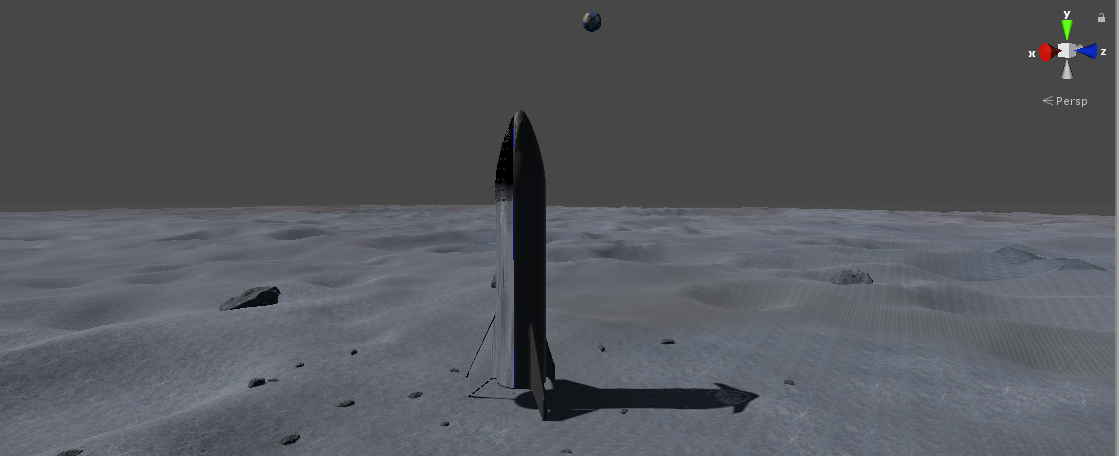
\includegraphics[width=0.85\textwidth]{VirgosRakete.PNG}
\caption{Die Rakete auf der Mondoberfläche}
\end{figure}

Innerhalb der Rakete befindet sich ein Kontrollraum, von dem aus man die Funktionen der Rakete steuern kann. Der Kontrollraum verfügt über zwei Türen und zwei Aufzüge, über die man die Rakete verlassen kann. Um die Türen zu öffnen muss zuerst die Luft aus dem Kontrollraum abgelassen werden. Dies geschieht über einen Knopf auf einer Schalttafel. Der Druckabfall wird durch eine Dämpfung der Umgebungsgeräusche simuliert. Anschließend kann eine der beiden Türen über einen anderen Knopf geöffnet werden. Zum Zeitpunkt der Entwicklung war nur eine der Türen und ein Aufzug funktionsfähig. Der Aufzug lässt sich über Knöpfe steuern die direkt am Aufzug angebracht sind. Über der Schalttafel der Rakete befinden sich drei Bildschirme. Zwei zeigen statische Bilder, während der Dritte eine Endlosschleife eines Videos abspielt. In der Mitte des Kontrollraums befindet sich ein Avatar in Form eines Astronauten, den der Spieler kontrolliert.\newline

\begin{figure}[H]
\centering
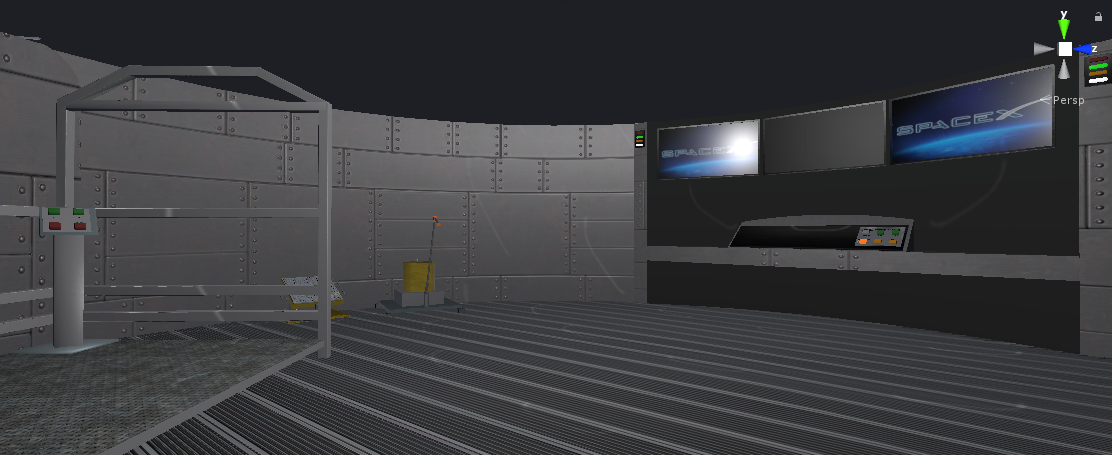
\includegraphics[width=0.85\textwidth]{VirgosKommandozentrale.PNG}
\caption{Der Kontrollraum in der Rakete}
\end{figure}

ViRGOS kann nur von einem Benutzer verwendet werden. Trotzdem verfügt die Anwendung über einen Voice-Chat, der die Kommunikation zwischen dem Benutzer in Virtual Reality und einem möglichen Außenstehenden ermöglicht. \\

Die zugehörige Hardware von ViRGOS setzt sich aus einem Virtual Reality Headset, zwei handgehaltenen Controllern, einem Virtualizer und dem Kransystem zusammen. Der Virtualizer ist ein Gerät das zur Lokomotion in Virtual Reality eingesetzt wird. Es ermöglicht dem Benutzer Bewegungen in alle Richtungen, ohne sich tatsächlich im Raum zu bewegen. Das Kransystem wird verwendet um einen Teil des Körpergewichtes des Benutzers aufzunehmen. Somit kann eine reduzierte Schwerkraft simuliert werden, was zur Immersion in die Weltraum-Umgebung beiträgt. 
 